\documentclass[10pt,letterpaper]{article}
\usepackage{tools}
\usepackage{enumitem}
%\settextfont{B Nazanin}
\usepackage{lipsum}
\setlength{\parskip}{3mm}
\setlength{\parindent}{0mm}
\newcommand{\wid}{0.49\textwidth}
\newcommand{\widone}{60mm}
\begin{document}
\Large
\begin{center}
In the name of beauty

4th problem set of ComNet course
\hl
\end{center}
Q1)

Determine the following statements as true or false. (Use enough reasons and explanation to support your answer)

\begin{enumerate}[label=\alph*-]
\item
Using TCP protocol we would have finer application-level control over what data is sent and when. 
%\item
%An application could have reliable data transfer while using UDP protocol.
\item
The length field in each UDP segment specifies the number of bytes in the UDP headers.
%\item
%If two UDP or TCP segments have different source IP addresses and/or source port numbers, but have the same destination IP address and destination port number, then the two segments will be directed to the same destination process via the same destination socket.
\item
Using less transmission rate in an end-to-end transmission, will increase sender utilization and effective throughput.
\item
Under rdt2.2 protocol in a channel with no packet loss, once the sender receives a corrupted packet from the receiver, it will wait until reception of a not corrupted packet from the receiver.
\end{enumerate}

Q2)

Assume a sender wishes to encapsulate the following message in a UDP segment:
\[
\begin{split}
&11001110
\\&00101011
\\&00011110
\\&10001111
\\&
\end{split}
\]
The checksum is calculated by the modulo 2 bitwise XOR of the above four 8bit strings in the message (the result is 8bit).
\begin{enumerate}[label=\alph*-]
\item
Determine the checksum the sender should calculate and append in the header.
\item
If the channel over which the segment should be sent, reverses each bit with a probability of $p$ independent of the others, calculate the probability that the receiver detects an error in the segment and drops it. Assume the error does not occur in the checksum field and it is the only header appended to the message.
\item
Calculate the probability of part b for a \textit{silent} error; i.e. when the message is corrupted but the error is not declared in the receiver. Calculate both of the probabilities of parts b- and c- for $p=0.01$.
\end{enumerate}

Q3)

Assume a sender uses rdt 3.0 (stop-and-wait) protocol to send packets to a receiver. Consider three senarios as described in Figure \ref{fig.1} where:
\begin{enumerate}[label=\alph*-]
\item
the packet with label \texttt{pkt1} is sent but lost due to link error. Assume the ACKs are never lost (Figure 3.a).
\item
the packet with label \texttt{pkt1} is sent by the sender and well received at the receiver but \texttt{ACK1} is lost due to link error. Assume the packets are never lost (Figure 3.b).
\item
the packet with label \texttt{pkt1} is sent but the sender uses an improper TIMEOUT interval. As a result, the TIMEOUT would be raised before the corresponding ACK for the sent packet is arrived at the sender. Assume the link is perfect and all the packets are never lost (Figure 3.c).
\end{enumerate}
Fully describe what instruction will the sender and receiver perform to make sure of perfect packet transmission under rdt3.0 protocol in each of the cases (a) to (c).

\begin{figure}[ht]
\centering
%%%%%%%%%%%%%%%%
\begin{subfigure}{\wid}
\centering
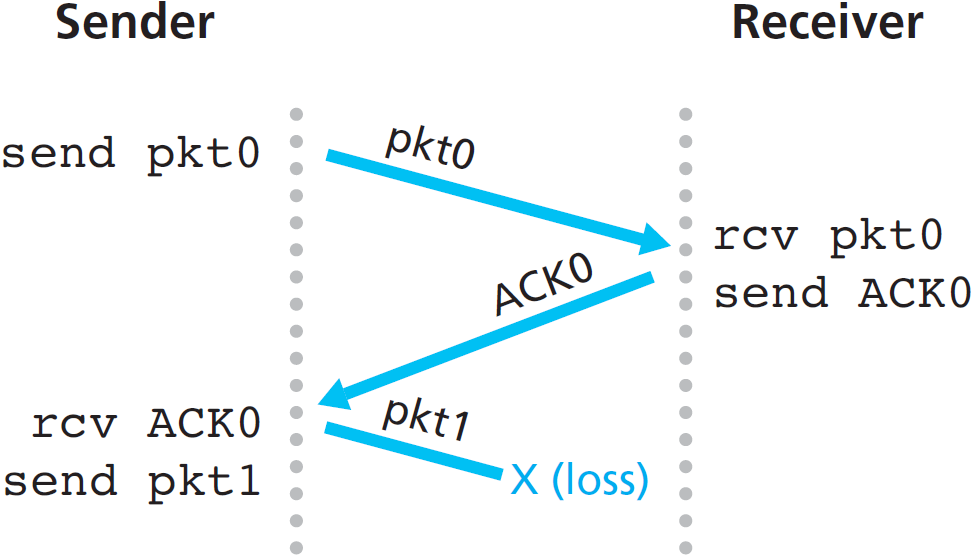
\includegraphics[width=\widone]{rdt1}
\caption{Packet Loss}
\end{subfigure}
%%%%%%%%%%%%%%%%
\begin{subfigure}{\wid}
\centering
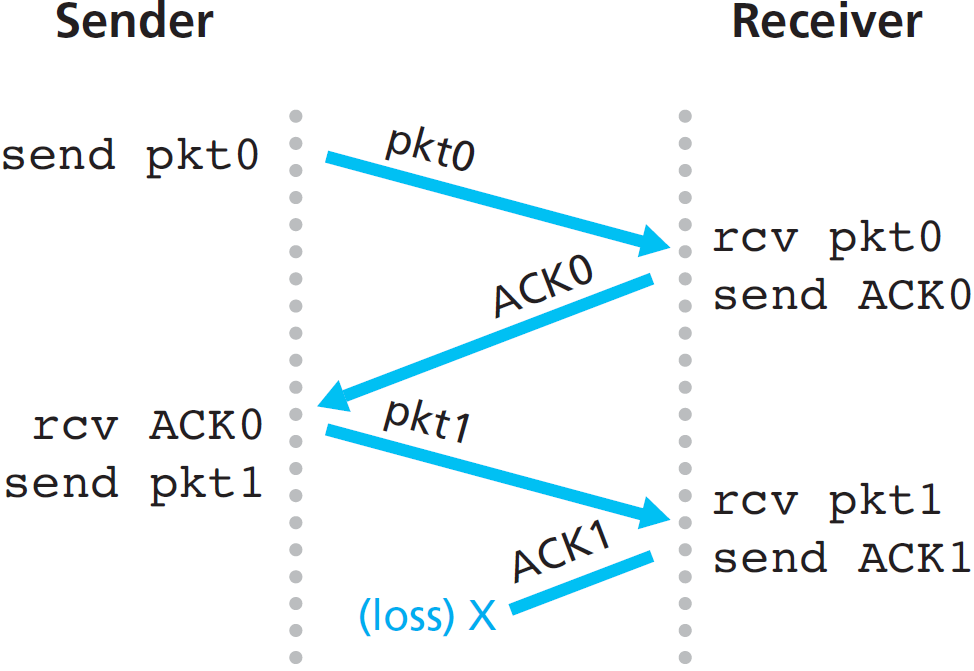
\includegraphics[width=\widone]{rdt2}
\caption{ACK Loss}
\end{subfigure}
%%%%%%%%%%%%%%%%
\begin{subfigure}{\wid}
\centering
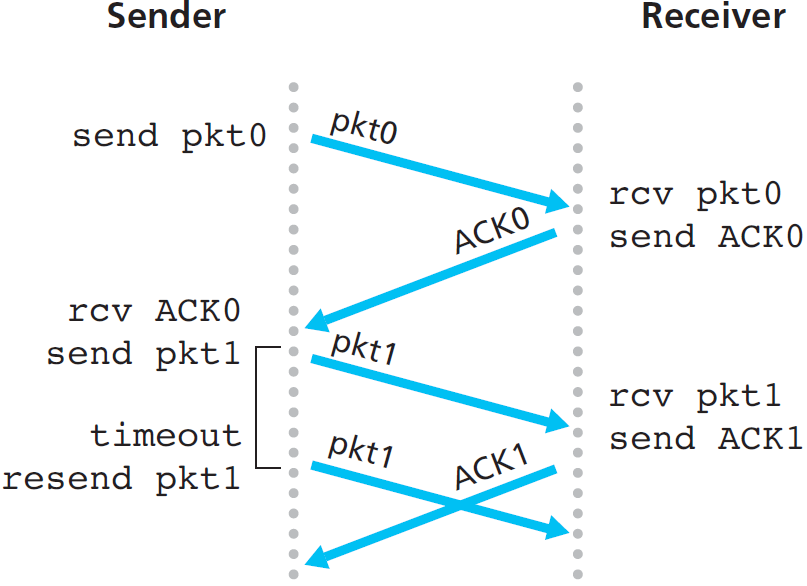
\includegraphics[width=\widone]{rdt3}
\caption{Improper TIMEOUT}
\end{subfigure}
%%%%%%%%%%%%%%%%
\caption{Three possible scenarios for rdt3.0 sender}
\label{fig.1}
\end{figure}

Q4)

Consider rdt 3.0 protocol in an ideal case, that is, with no bit error or loss. The sender transmits $n$ packets consecutively using pipelining. Assume $L=500$ bytes is the packet size, $R=4\text{Gbps}$ is the transmission rate, the distance between sender and receiver is 1000 km and the propagation speed is $2\times 10^8$ m/s. Suppose the ACK messages will not suffer transmission time due to small packet size.

\begin{enumerate}[label=\alph*-]
\item
Calculate the sender utilization and the effective end-to-end throughput for general values of $n$.
\item
How much would the sender utilization and the effective throughput be if $n=1$ (no pipelining)? Will exploiting a link with lower transmission rate be a good idea from the aspect of utilization and effective throughput improvement? Why or why not?
\item
How much would the traffic utilization be at the sender side if $n=8$?
\end{enumerate}
%\newpage
%$$
%{nL/R\over nL/R+0.01}={nL\over nL+0.01\times R}R
%$$
%
%$$
%{nL\over }
%$$
%\newpage

Q5)

Consider the Finite State Machine of protocol rdt2.1 as shown in Figures 2 and 3. Since the protocol of rdt2.1 generally works well with a channel with no packet loss, add a TIMEOUT to both the sender side and receiver side of rdt2.1 so as to avoid the infinity loop of waiting for lost packets (draw the modified FSM for both the sender side and receiver side).
\begin{figure}[ht]
\centering
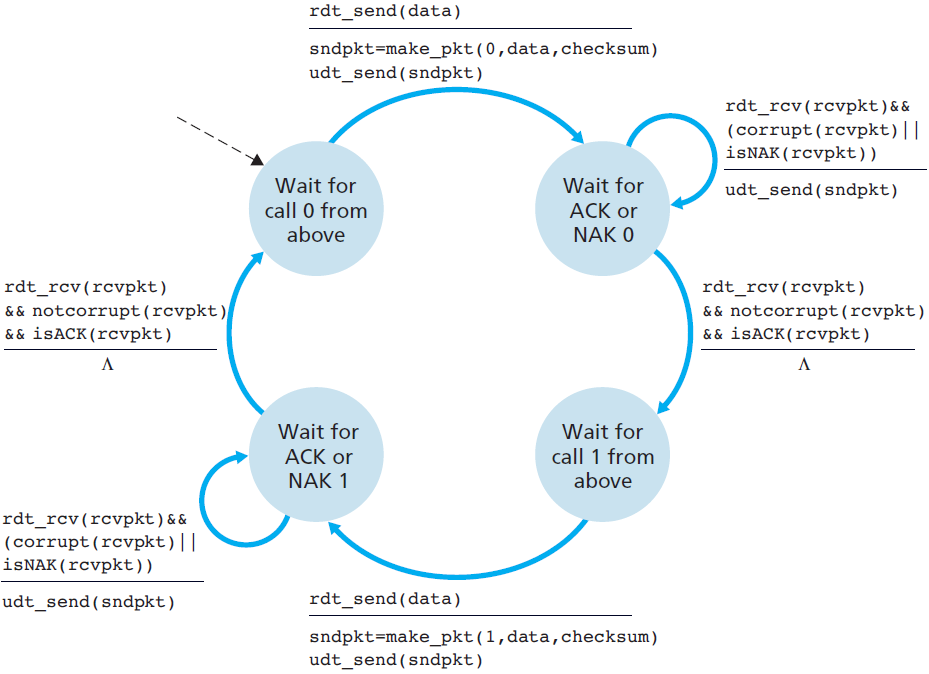
\includegraphics[width=150mm]{rdtsender}
\caption{rdt2.1 sender}
\end{figure}
\begin{figure}[ht]
\centering
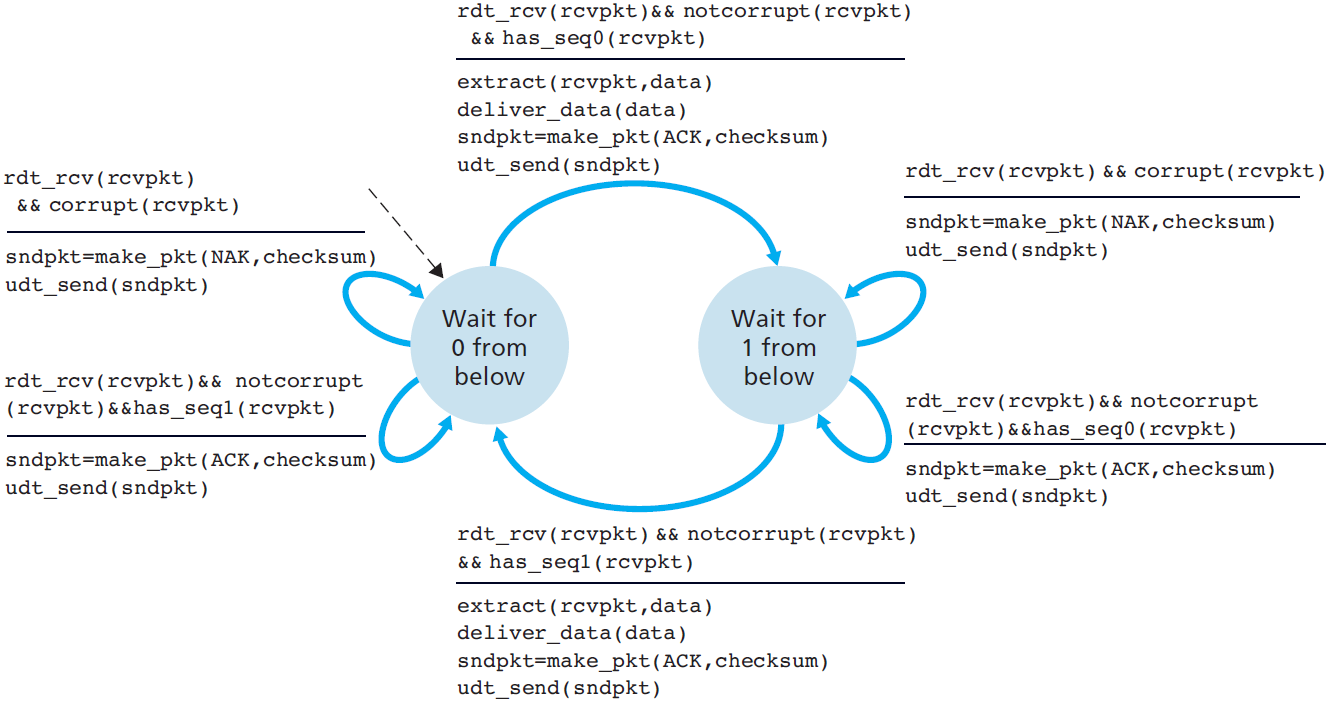
\includegraphics[width=150mm]{rdtrecv}
\caption{rdt2.1 receiver}
\end{figure}
%Determine the following statements as true or false with enough reasons.
%\begin{enumerate}[label=\alph*-]
%\item
%Both trasport and network layer protocols provide logical communication between processes running at different hosts rather than hosts themselves.
%\item
%Transport layer packets are refered to as \textbf{datagrams}.
%\item
%TCP ensures that the transmitted packets would finally reach their destination, however it makes no guarantee on the order of packets.
%\item
%The IP service model is a best-effort delivery service since it guarantees to deliver segments between communicating hosts, whether orderless or not.
%%\item
%%Cookies are used to keep track of user IDs in a stateless HTTP server.
%%\item
%%Link-layer switches are typically capable of processing the packets up to the layer 3.
%%\item
%%SMTP and FTP are examples of layer 1 protocols while TCP is a transport layer protocol.
%%\item
%%API is a set of rules 
%%\item
%%For economical reasons, exploiting optical fibers is not recommended in long-haul network
%\end{enumerate}
%
%Q2)
%\begin{enumerate}[label=\alph*-]
%\item
%Why is IP said to be an unreliable service and if so, how would TCP provide reliable data transfer on top of IP?
%\item
%Why are source and destination host port numbers included in segment headers? What problem could arise if they are ignored?
%\end{enumerate}
%
%Q3) Suppose Client A initiates a Telnet session with Server S. At about the same
%time, Client B also initiates a Telnet session with Server S. Provide possible
%source and destination port numbers for
%\begin{enumerate}[label=\alph*-]
%\item
%The segments sent from A to S.
%\item
%The segments sent from B to S.
%\item
%The segments sent from S to A.
%\item
%The segments sent from S to B.
%\item
%If A and B are different hosts, is it possible that the source port number in
%the segments from A to S is the same as that from B to S?
%\item
%How about if they are the same host?
%\end{enumerate}
%(Choose the port numbers at source and destination arbitrarily.)
%
%Q4) Consider the following Figure. What are the source and destination port values in the segments
%flowing from the server back to the clients’ processes? What are the IP
%addresses in the network-layer datagrams carrying the transport-layer segments?
%\begin{figure}[ht]
%\centering
%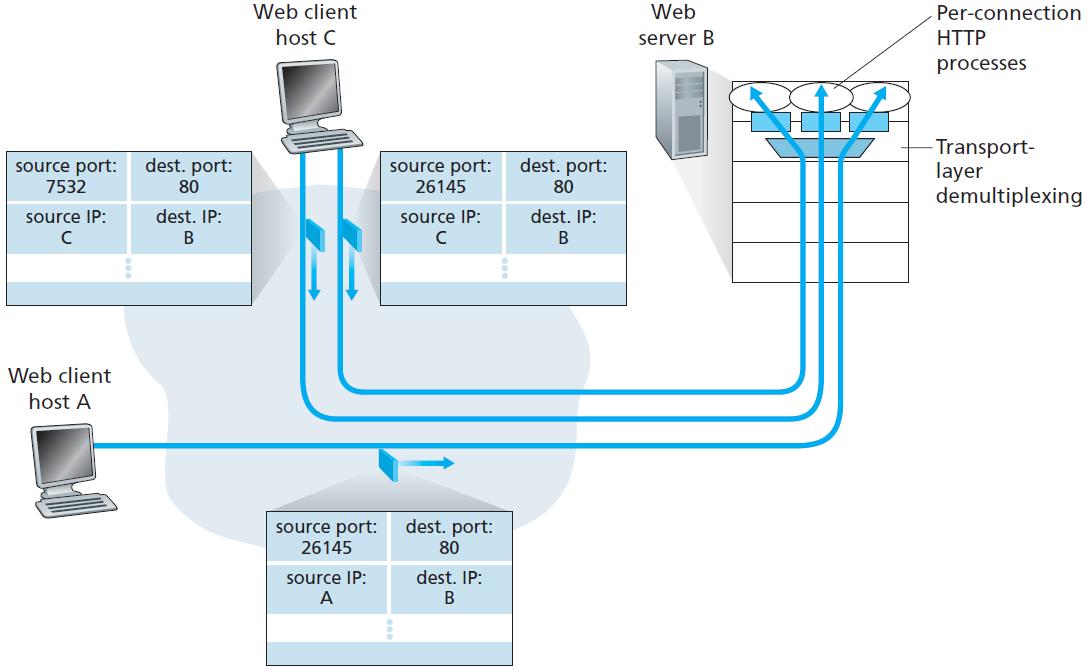
\includegraphics[width=180mm]{simnet}
%\end{figure}
\end{document}